\documentclass[a4paper,12pt]{toptesi}

\usepackage{hyperref}
\usepackage{amsmath}
\usepackage{amsthm}
\usepackage{enumitem}
\usepackage{listings}
\usepackage{xcolor}

\hypersetup{
    pdfpagemode={UseOutlines},
    bookmarksopen,
    pdfstartview={FitH},
    colorlinks,
    linkcolor={black},
    citecolor={black},
    urlcolor={black}}
  
\colorlet{punct}{red!60!black}
\definecolor{background}{HTML}{EEEEEE}
\definecolor{delim}{RGB}{20,105,176}
\colorlet{numb}{magenta!60!black}

\theoremstyle{definition}
\newtheorem{defn}{Definizione}

\lstdefinelanguage{json}{
    basicstyle=\footnotesize\ttfamily,
    numbers=left,
    numberstyle=\scriptsize,
    stepnumber=1,
    numbersep=8pt,
    showstringspaces=false,
    breaklines=true,
    frame=lines,
    backgroundcolor=\color{background},
    literate=
      {:}{{{\color{punct}{:}}}}{1}
      {",}{"{{\color{punct}{,}}}}{1}
      {\{}{{{\color{delim}{\{}}}}{1}
      {\}}{{{\color{delim}{\}}}}}{1}
      {[}{{{\color{delim}{[}}}}{1}
      {]}{{{\color{delim}{]}}}}{1}}

\ateneo{\href{http://www.uniba.it/}{Universit{\`a} degli Studi di Bari}}
\nomeateneo{\href{http://www.uniba.it/}{``Aldo Moro''}}
\FacoltaDi{Dipartimento di Informatica}
\CorsoDiLaureaIn{Corso di Laurea Triennale in }
\corsodilaurea{Informatica}
\TesiDiLaurea{Tesi di Laurea }
\materia{Metodi Avanzati di Programmazione}
\titolo{Analisi di Social Media per la Scoperta di Pattern di Interazione}
\logosede{img/sigillo}
\relatore{\tabular{@{}l@{}}
dr.\ Corrado Loglisci \\
prof.\ Donato Malerba \\ [1.5ex]
\textbf{Correlatore:} \\
dott.\ Angelo Impedovo
\endtabular}
\candidato{\tabular{@{}l@{}} {Donato Meoli} \endtabular}
\def\Candidato{Laureando}
\sedutadilaurea{\textsc{Anno~accademico} 2016-2017}

\begin{document}

\frontespizio

\begin{citazioni}
	\textit{La dignit{\`a} non consiste nel possedere onori, ma nella coscienza di meritarli. \\}
    \textsc{Aristotele}
\end{citazioni}

\sommario
Obiettivo generale del presente progetto {\`e} quello di realizzare strumenti computazionali in grado di modellare comunit{\`a} collaborative attraverso l'analisi di dati, prodotti e memorizzati dalle medesime comunit{\`a}. In un contesto fortemente caratterizzato dall'interazione tra gli uomini, bench{\`e} mediata da tecnologie, una comunit{\`a} rappresenta un dominio che evolve nel tempo, i cui cambiamenti possono essere molteplici e possono riguardare fattori interni o esterni alla comunit{\`a}. Lo studio dei cambiamenti diventa cruciale per caratterizzare l'evoluzione della comunit{\`a} e modellarla, quindi, in maniera completa. A tal proposito si condurr{\`a} una attivit{\`a} mirata a sintetizzare metodi di analisi che siano in grado di scoprire le interazioni tra partecipanti, a partire da dati riguardanti relazioni sociali tra questi. Molte delle informazioni di una comunit{\`a} sono prodotte in forma non strutturata e  in linguaggio naturale. Tipicamente, la loro comunicazione avviene tramite strumenti di messaggistica istantanea o su forum di discussione tematici. Questo significa che molte delle informazioni assunte non sono apertamente esplicitate e direttamente accessibili, ma riportate in testo scritto. Nasce quindi la necessit{\`a} di investigare su approcci di elaborazione del linguaggio naturale per l'identificazione di relazioni tra i partecipanti.

\figurespagetrue
\indici

\renewcommand\lstlistlistingname{Elenco dei Listati}
\lstlistoflistings

\part{Contesto \& Obiettivi}

\include{capitoli/01_ComunitàOnline}

\part{Costruzione di Grafi da Social Media}
\chapter{Estrazione di Grafi Basati sul Contenuto}

\section{Pipeline di Elaborazione del Linguaggio Naturale sul Contenuto}

Il natural language processing {\`e} una branca dell'intelligenza artificiale che concerne l'elaborazione automatica del linguaggio naturale. Trattandosi di un processo particolarmente complesso a causa delle caratteristiche intrinseche di ambiguit{\`a} del linguaggio umano, tra cui sinonimia e polisemia, esso viene suddiviso in fasi diverse. Lo scopo {\`e} quello di determinare la funzione delle singole parole, che vengono suddivise in classi sintattiche (nomi, verbi, aggettivi e avverbi), in base alla loro funzione all'interno di una frase.

Lo Stanford NLP\footnote{Natural Language Processing} Group {\`e} uno dei gruppi di ricerca di maggiore importanza nel settore dell'elaborazione del linguaggio naturale ed offre validi strumenti per realizzare tale scopo. Attraverso le \href{https://github.com/stanfordnlp/CoreNLP}{API Java} del modulo software \href{https://stanfordnlp.github.io/CoreNLP/}{CoreNLP} {\`e} possibile analizzare il dataset corpus per poter distinguerne le parole (tokenization), lemmatizzarle, nonch{\`e} ridurle alla loro forma canonica, e determinarne la funzione (PoS\footnote{Part of Speech} tagging) all'interno della frase. {\`E} cos{\`i} possibile classificarle nelle categorie sintattiche di nostro interesse che includono:

\paragraph{Nomi}

\begin{enumerate}[label=(\roman*)]
  
\item \textit{NN}: singolare;
\item \textit{NNP}: proprio singolare;
\item \textit{NNS}: plurale;
\item \textit{NNPS}: proprio plurale.

\end{enumerate}

\paragraph{Verbi}

\begin{enumerate}[label=(\roman*)]
  
\item \textit{VB}: forma base;
\item \textit{VBD}: passato;
\item \textit{VBG}: gerundio o participio presente;
\item \textit{VBN}: participio passato;
\item \textit{VBP}: presente singolare (esclusa terza persona singolare);
\item \textit{VBZ}: presente, terza persona singolare.

\end{enumerate}

\begin{figure}\centering
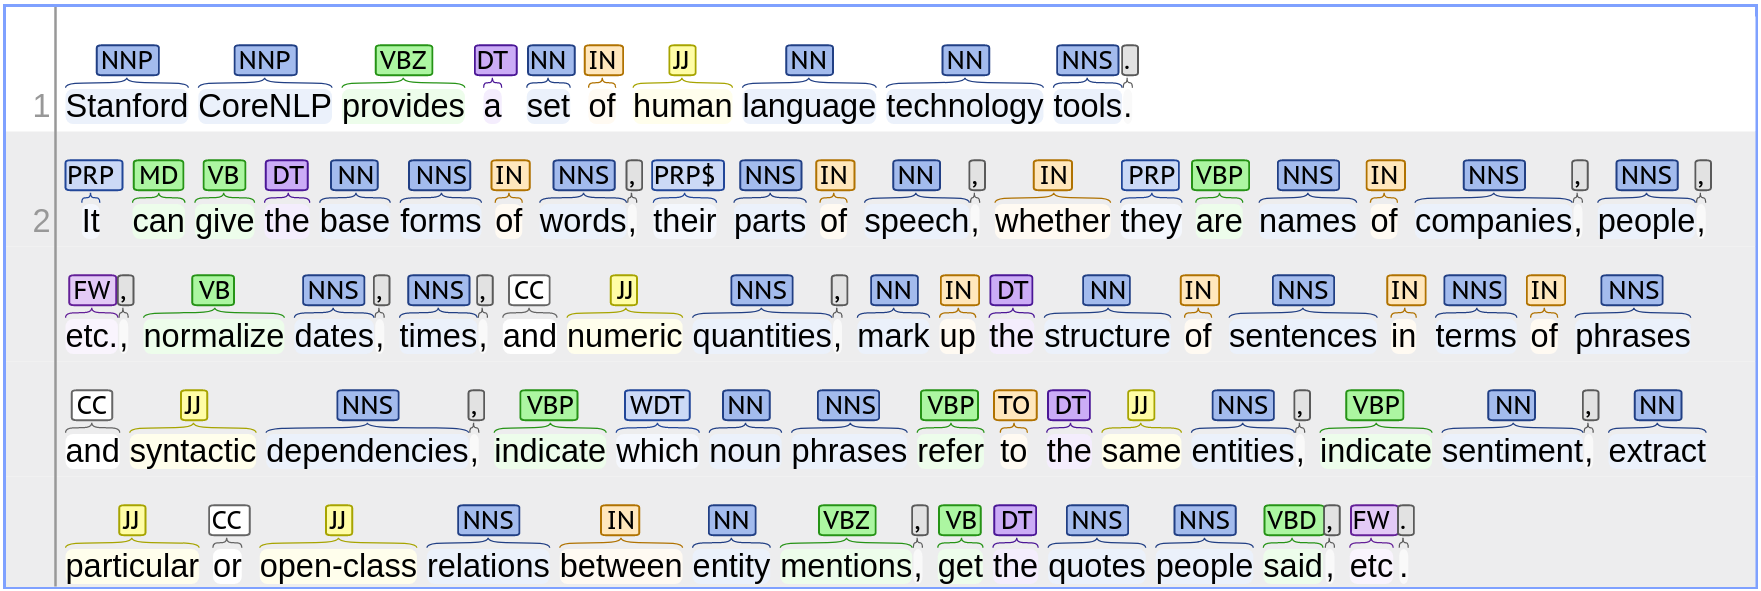
\includegraphics[scale=0.20]{img/pos}
\caption{Esempio di part-of-speech tagging.}
\end{figure}

\section{Identificazione di Archi Basati su Similarit{\`a}}
Il risultato della fase di NLP, costituita dai verbi e dai nomi lemmatizzati, si presta ad essere utilizzato per l'estrazione di caratteristiche linguistiche.

\subsection{Archi Basati su Similarit{\`a} Lessicale}
La similarit{\`a} lessicale tra i messaggi {\`e} stata calcolata grazie ad una versione modificata del Lexical Match Algorithm (LMA) \cite{hic} che considera i messaggi che si presuppone possano essere simili. Il LMA integra il Vector Space Model (VSM), nonch{\`e} uno dei pi{\`u} popolari metodi usati per identificare somiglianze lessicali. La formula del LMA per calcolare la similarit{\`a} lessicale produce un valore compreso tra 0 e 1 e pu{\`o} essere formalizzata come segue:

\begin{equation}
\sum_{i=0}^{LenX} {\sum_{j=0}^{LenY}}_{if POS(X_{i}) = POS(Y_{j})} \frac{TF_{X_{i}} + TF_{Y_{j}}}{DF_{X_{i}} + DF_{Y_{j}}} \cdot (LenX \cdot LenY)^{-1}
\end{equation}

dove: 

\begin{enumerate}[label=(\roman*)]
  
\item \( X \) ed \( Y \) sono i due messaggi;
\item \( LenX \) e \( LenY \) sono il numero di verbi e nomi contenuti rispettivamente nei messaggi \( X \) ed \( Y \);
\item \( POS \) {\`e} il part-of-speech tag;
\item \( X_{i} \) ed \( Y_{j} \) si riferiscono rispettivamente agli i-esimi e j-esimi nomi o verbi lemmatizzati contenuti nei messaggi \( X \) ed \( Y \);
\item \( TF \) {\`e} il term frequency e \( DF \) {\`e} il document frequency.

\end{enumerate}

\subsection{Archi Basati su Similarit{\`a} Semantica}
La similarit{\`e} semantica {\`e} una metrica definita su un insieme di documenti o termini, in cui l'idea della distanza tra loro si basa sulla similarit{\`a} del loro significato o contenuto semantico rispetto alla similarit{\`a} che pu{\`o} essere stimata per quanto riguarda la loro rappresentazione sintattica. Questi sono strumenti matematici usati per stimare la forza della relazione semantica tra unit{\`a} di linguaggio, concetti o istanze, attraverso una descrizione numerica ottenuta in base al confronto di informazioni che supportano il loro significato o descrivono la loro natura. Il termine similarit{\`a} semantica è spesso confuso con la relazione semantica. La relazione semantica include qualsiasi relazione tra due termini, mentre la similarit{\`a} semantica include solo le relazioni "is a".

Computazionalmente, la similarit{\`a} semantica può essere stimata definendo una similarit{\`a} topologica, utilizzando le ontologie per definire la distanza tra termini/concetti. Ad esempio, una metrica per il confronto di concetti ordinati in un insieme parzialmente ordinato e rappresentati come nodi di un grafo aciclico e diretto (ad esempio una tassonomia), sarebbe il percorso pi{\`u} breve che collega i due nodi concettuali. Sulla base di analisi testuali, la correlazione semantica tra unit{\`a} linguistiche pu{\`o} anche essere stimata utilizzando mezzi statistici come il VSM \footnote{Vector Space Model} per correlare parole e contesti testuali da un corpus testuale adatto.

Il concetto di similarit{\`a} semantica {\`e} pi{\`u} specifico della relazione semantica, in quanto quest'ultimo include concetti come l'antonimia e la meronimia, mentre la similarit{\`a} no. Tuttavia, gran parte della letteratura usa questi termini in modo intercambiabile, insieme a termini come la distanza semantica. In sostanza, la similarit{\`a} semantica, la distanza semantica e la relazione semantica hanno in comune il fatto che il loro risultato {\`e} solitamente un valore compreso tra -1 e 1 o tra 0 e 1, dove 1 indica una similarit{\`a} estremamente alta.

Nel modello proposto in questa tesi, la similarit{\`a} semantica tra i messaggi viene calcolata, utilizzando l'ontologia linguistica \href{https://wordnet.princeton.edu/}{WordNet} 3.0, attraverso la formula di similarit{\`a} di Lin (1998) \cite{lin}, implementata dalle \href{https://code.google.com/archive/p/ws4j/}{API WS4J} (WordNet Similarity for Java). La similarit{\`a} di Lin {\`e} compresa tra 0 e 1 e pu{\`o} essere espressa in maniera formale come segue:

\begin{equation}
\label{eq:5.2}
lin(x,y) = \frac{2 \cdot \sum_{t \in syn(x) \cap syn(y)} log P(t)}{\sum_{t \in syn(x)} log P(t) + \sum_{t \in syn(y)} log P(t)}
\end{equation}

dove:

\begin{enumerate}[label=(\roman*)]
  
\item \( x \) ed \( y \) sono due parole;
\item \( syn \) {\`e} il synset;
\item \( P(t) \) {\`e} la probabilit{\`a} del termine \( t \).

\end{enumerate}

Il risultato della formula di similarit{\`a} Lin {\`e} stato poi pesato con i TFIDF (term frequency - inverse document frequency) delle stesse per far si che i termini pi{\`u} frequenti, e quindi semanticamente meno discriminanti, abbiano un'incidenza minore sul valore finale. Quindi, dati due messaggi, la formula per il calcolo della similarit{\`a} semantica {\`e} la seguente: 

\begin{equation}
\sum_{i=0}^{LenX} {\sum_{j=0}^{LenY}}_{if POS(X_{i}) = POS(Y_{j})} \frac{lin(X_{i},Y_{j}) \cdot \frac{TFIDF(X_{i}) + TFIDF(Y_{j})}{2}}{\sum_{t \in X \cup Y} TFIDF(t)}
\end{equation}

\begin{enumerate}[label=(\roman*)]
  
\item \( X \) ed \( Y \) sono i due messaggi;
\item \( LenX \) e \( LenY \) sono il numero di verbi e nomi contenuti rispettivamente nei messaggi \( X \) ed \( Y \);
\item \( POS \) {\`e} il part-of-speech tag;
\item \( X_{i} \) ed \( Y_{j} \) si riferiscono rispettivamente agli i-esimi e j-esimi nomi o verbi lemmatizzati contenuti nei messaggi \( X \) ed \( Y \);
\item \( lin \) {\`e} la similarit{\`a} di Lin definita dalla formula \eqref{eq:5.2};
\item \( TFIDF \) {\`e} il term frequency - inverse document frequency.

\end{enumerate}

\chapter{Modellazione dei Grafi}

Le comunit{\`a} analizzate prevedono relazioni tra gli utenti che sono supportate dagli strumenti tecnologici in uso, piuttosto che essere identificate a priori per via delle relazioni sociali che intercorrono tra questi, come nel caso di ``follow" o ``amicizia". 

La struttura dati che si presta meglio alla rappresentazione di un dominio applicativo di questo tipo {\`e} sicuramente un grafo in cui i nodi rappresentano gli utenti e gli archi corrispondono alle relazioni che intercorrono tra di loro.

La fase di costruzione del grafo come astrazione della comunit{\`a} da analizzare nel prossimo step prevede la rappresentazione di ben 5 diverse tipologie di relazioni possibili che possono intercorrere tra gli utenti. Le prime 3 sono basate su delle banali relazioni sociali immediatamente disponibili, in quanto deducibili dalla struttura multi-threading implementata dalla maggior parte delle tecnologie che supportano le comunit{\`a} sociali. Le altre 2, invece, sono basate sul contenuto dei messaggi che gli utenti hanno scambiato all'interno di uno stesso forum di discussione, ossia sulle similarit{\`a} lessicali e semantiche calcolate come descritto nel capitolo precedente.

Il risultato sar{\`a} quindi un grafo orientato, etichettato e pesato con gli score di similarit{\`a} per gli archi che rappresentano tale tipologia di relazione.

% \begin{figure}\centering
% \includegraphics[scale=0.25]{img/graph-all}
% \caption{Porzione del grafo rappresentante tutte le possibili tipologie di relazioni che possono presentarsi tra gli utenti.}
% \end{figure}

\subparagraph{COMMENT\_TO}
{\`E} una delle relazioni pi{\`u} semplici che pu{\`o} intercorrere tra due nodi del grafo: un utente \( b \) commenta il post di un utente \( a \). 

% \begin{figure}\centering
% \includegraphics[scale=0.25]{img/graph-comment}
% \caption{}
% \end{figure}

\subparagraph{REPLY\_TO} 
Prevede la replica di un utente \( c \) al commento dell'utente \( b \) sul post dell'utente \( a \).

% \begin{figure}\centering
% \includegraphics[scale=0.25]{img/graph-reply}
% \caption{}
% \end{figure}

\subparagraph{MENTION\_TO}
Comporta la creazione di un link tra un utente \( s \) ed un utente \( m \) oggetto del menzionamento, anche se coinvolti in forum o thread di discussione diversi.

% \begin{figure}\centering
% \includegraphics[scale=0.25]{img/graph-mention}
% \caption{}
% \end{figure}

\subparagraph{LEXICALLY\_SIMILAR\_TO}
{\`E} dovuta alla similarit{\`a} lessicale tra post di due utenti coinvolti nella stessa discussione, la cui direzionalit{\`a} dell'arco {\`e} definita in base al timestamp.

% \begin{figure}\centering
% \includegraphics[scale=0.25]{img/graph-lexical}
% \caption{}
% \end{figure}

\subparagraph{SEMANTICALLY\_SIMILAR\_TO}
{\`E} dovuta alla similarit{\`a} semantica tra post di due utenti coinvolti nella stessa discussione, la cui direzionalit{\`a} dell'arco {\`e} decisa in base al timestamp.

% \begin{figure}\centering
% \includegraphics[scale=0.25]{img/graph-semantic}
% \caption{}
% \end{figure}


\part{Analisi di Grafi Costruiti da Social Media}
\chapter{Analisi di Dati Temporali}

La neccessit{\`a} di trarre conclusioni incrementali per quanto riguarda i dati presenti in uno stream spesso non {\`e} soddisfacibile. Sebbene l'idea chiave risulti ancora oggi abbastanza vincente, tuttavia, la ricorsivit{\`a} non {\`e} caratteristica comune a tutti i problemi che si vorrebbero affrontare sui dati provenienti da uno stream: molti problemi hanno bisogno di processare necessariamente un insieme di dati per volta, con le dovute complicazioni in termini di consumi e performance.

La letteratura ha fornito diversi esempi di modelli per l'analisi progressiva dei data stream, probabilmente quello pi{\`u} vincente {\`e} sicuramente il modello basato sulle finestre temporali (time windows).

Una finestra temporale {\`e}, intuitivamente, una partizione dell'asse temporale, di ampiezza fissa o variabile, a partire da un determinato punto temporale.

\begin{defn}
Si definisce finestra temporale $W(t,\Delta t)$, che comincia all'istante \( t \) con un'ampiezza $\Delta t$, come l'intervallo di tempo intercorrente fra l'istante \( t \) e l'istante $t+\Delta t$.
\end{defn}

La finestra temporale, appena definita in accezione puramente temporale, solitamente sottende una partizione sui dati in ingresso che sono time-stamped. Se, ad esempio, avessimo un data stream caratterizzato alla maniera seguente:

\begin{equation}
DS = \lbrace (d_1,t_1),(d_2,t_2),(d_3,t_3),(d_4,t_4),(d_5,t_5) \rbrace
\end{equation}
 
ossia un data stream che ha ricevuto soltanto 5 dati \( (d_i) \) in altrettanti istanti temporali \( (t_i) \) differenti, allora la finestra temporale \( W(2,2) \) risulta essere come segue:

\begin{equation}
W(2,2) = \lbrace(d_2,t_2),(d_3,t_3)\rbrace
\end{equation}

{\`E} facile capire come $W(t,\Delta t)$ induca sempre l'individuazione di un sottinsieme di \( DS \); occorre pertanto dare una definizione operativa di finestra temporale in funzione di un data stream associato.

\begin{defn}
Si definisce finestra temporale associata al data sream \( DS \), a partire dall'istante \( t \) con un'ampiezza $\Delta t$, come il sottinsieme dei dati presenti nel data stream il cui istante di arrivo {\`e} compreso nell'intervallo $[t,\Delta t]$

\begin{equation}
W(DS,t,\Delta t) = \lbrace (d_i,t_i) \in DS \mid t_i \in [t,\Delta t]\rbrace
\end{equation}
\end{defn}

In quest'ottica operativa vale sempre la propriet{\`a} secondo cui \\ $W(DS,t,\Delta t) \subseteq DS$.

Questa definizione generale di finestra temporale, in realt{\`a}, nasconde tutta una serie di modelli di finestre temporali derivate a partire dal concetto base.

Esistono modelli che consentono ad alcune delle variabili indipendenti $(DS,t,\Delta t)$ di variare nel tempo: una finestra temporale infatti, a seconda del modello considerato, pu{\`o} traslare in avanti nel tempo, variare la propria ampiezza o addirittura fare entrambe le cose.

\section{Landmark Windows}

Il modello temporale di tipo landmark afferisce ad una particolare tipologia di finestre temporali $W(DS,t,\Delta t)$ in cui il parametro di ampiezza $\Delta t$ pu{\`o} aumentare nel tempo. Questo tipo di finestra temporale ha la particolare inefficienza di crescere di dimensione nel tempo ($\Omega(\Delta t)$ dati dove $\Delta t$ {\`e} l'ampiezza iniziale), se non limitata, rendendo potenzialmente inefficiente (in base alla quantit{\`a} di dati esibiti) qualsiasi algoritmo che non scala in maniera adeguata.

\begin{figure}\centering
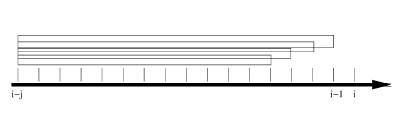
\includegraphics[scale=0.70]{img/landmark-windows}
\caption{Una landmark window che cresce fino all'instante temporale \( i-1 \).}
\end{figure}

Le finestre temporali di tipo landmark, tuttavia, hanno provato la loro efficacia nel risolvere quei problemi incrementali, specie in quelli dove c'{\`e} un uso abbondante di ``blocking operations" oltre ad un'assenza di ricorsivit{\`a}. 

Ai fini della tesi in esame, questa finestra temporale crescente nel tempo riveste un interesse particolare in quanto ci permetter{\`a} di adempiere agli obbiettivi prefissati, ossia quello di investigare lo studio dei cambiamenti della comunit{\`a} per caratterizzare l'evoluzione attraverso la scopera di interazioni tra i partecipanti.

% \section{Grafo Temporale}


% \subsection{Grafo Temporale Cumulativo}

% \begin{figure}\centering
% 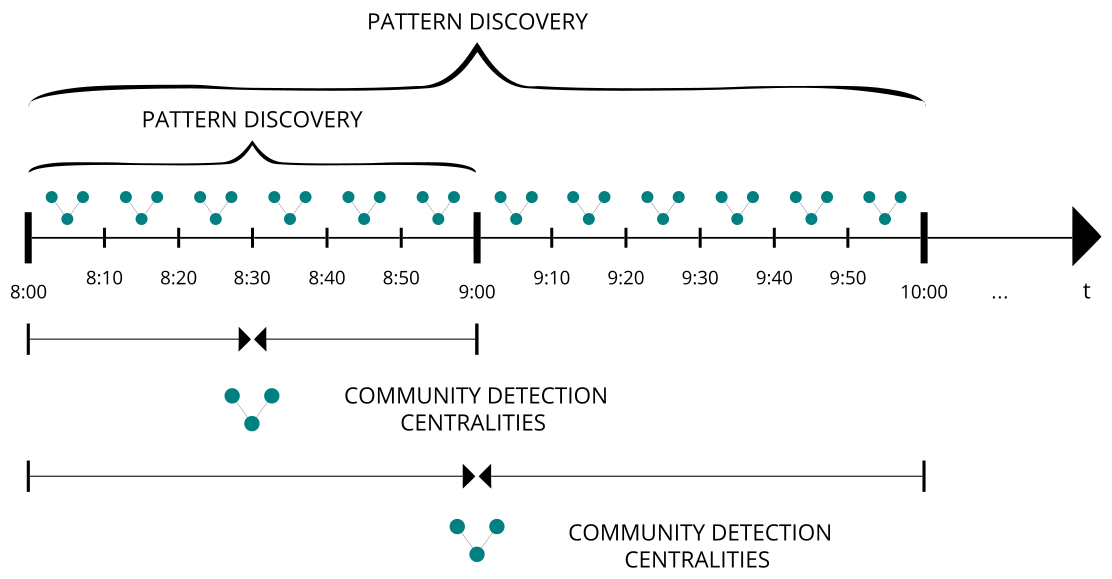
\includegraphics[scale=0.30]{img/temp-graph}
% \caption{.}
% \end{figure}
\chapter{Analisi di Dati in Forma di Grafo}

Nell'analisi dei social networks, i concetti di teoria dei grafi vengono utilizzati per capire e spiegare i fenomeni sociali.

Gli algoritmi sui grafi vengono utilizzati per calcolare metriche riguardo nodi e relazioni. Possono fornire informazioni su entit{\`a} rilevanti nel grafo, esprimibili in termini di indicatori di centralit{\`a}, o strutture intrinseche come comunit{\`a} per mezzo di metodi di partizionamento o clustering. Molti di questi approcci attraversano frequentemente il grafo per il calcolo di tali metriche, eseguendo ricerche in ampiezza o in profondit{\`a}, per cui, a causa della crescita esponenziale dei possibili cammini, molti approcci hanno anche un'elevata complessit{\`a} algoritmica. Per questo motivo, al fine di eseguire un'analisi efficiente dei grafi temporali cumulativi, sono state utilizzate le \href{https://github.com/neo4j-contrib/neo4j-graph-algorithms}{API} di neo4j, ottimizzate in quanto utilizzano determinate strutture del grafo, memorizzano parti gi{\`a} esplorate e parallelizzano le operazioni.

\section{Ruolo dell'Utente: Indicatori di Centralit{\`a}}

Uno strumento essenziale ed efficace per l'analisi dei social networks {\`e} costituito dagli indicatori di centralit{\`a} definiti sui nodi (Bavelas, 1948 \cite{Bavelas-centrality}; Sabidussi, 1966 \cite{Sabidussi-centrality}; Freeman, 1979 \cite{Freeman-centrality}) e  progettati per classificarli in base alla loro posizione nel grafo.

\subsection{Centralit{\`a} ``Degree"}

La centralit{\`a} ``degree'' di un nodo {\`e} data dal numero delle relazioni in cui esso {\`e} coinvolto ed {\`e} una misura di centralit{\`a} semplice ma efficace che fornisce un grado di importanza nodale. Pi{\`u} alto sar{\`a} il suo valore, pi{\`u} esso ricoprir{\`a} un ruolo importante nel grafo. 

In un grafo orientato come quello sociale in questione, per il calcolo di tale indicatore si fa una distinzione in base al fatto che un nodo sia coinvolto in una relazione in entrata o in uscita. Tali valori prendono rispettivamente il nome di \textbf{in-degree} ed \textbf{out-degree} e sono utili per mettere in evidenza il ruolo di alcuni nodi nel grafo come attrattori o mittenti. I nodi hub hanno un degree elevato, al pi{\`u} ugule alla somma di tutti i degree degli altri nodi del grafo, mentre i nodi spoke hanno un degree almeno pari ad 1. 

\begin{defn}
Sia \( G = (V,A) \) un grafo orientato dove \( V \) {\`e} l'insieme dei vertici ed \( A \) l'insieme degli archi, le centralit{\`a} ``in-degree'' ed ``out-degree'' possono essere definite rispettivamente come segue:

\begin{equation}
{C_D}^+(v) =  \sum_{\substack{a \in A \\ s \in V}} a_{sv}
\end{equation}

\begin{equation}
{C_D}^-(v) =  \sum_{\substack{a \in A \\ s \in V}} a_{vs}
\end{equation}

dove \( a_{sv} \) {\`e} l'arco che va dal nodo \( s \) al nodo \( v \) e viceversa.
\end{defn}

\subsection{Centralit{\`a} ``Betweenness"}

La centralit{\`a} ``betweenness'' (Anthonisse, 1971 \cite{Anthonisse-betweenness}; Freeman, 1977 \cite{Freeman-betweenness}) {\`e} una misura di centralit{\`a} basata sul calcolo dei cammini minimi ed {\`e} utile per trovare i nodi che fungono da ponte da una parte all'altra del grafo.

Per ogni coppia di nodi in un grafo connesso, esiste almeno un percorso pi{\`u} breve che pu{\`o} essere basato sul numero di relazioni che il percorso attraversa, se il grafo non {\`e} pesato, o sulla somma dei pesi delle relazioni, in caso contrario. Tale indicatore viene calcolato sommando, per ciascun nodo, il numero di percorsi pi{\`u} brevi che lo attraversano. I nodi che si trovano pi{\`u} frequentemente su questi percorsi avranno un punteggio di centralit{\`a} pi{\`u} elevato. 

\begin{defn}
Sia \( G = (V,A) \) un grafo orientato dove \( V \) {\`e} l'insieme dei vertici ed \( A \) l'insieme degli archi, la centralit{\`a} ``betweenness'' di un vertice \( v \) {\`e} definita come segue:

\begin{equation}
C_B(v) = \sum_{s \neq v \neq t \in V} \frac{\sigma_{st}(v)}{\sigma_{st}}
\end{equation}

dove:

\begin{enumerate}[label=(\roman*)]
  
\item \( \sigma_{st}(v) \) {\`e} il numero totale di percorsi minimi dal nodo \( s \) al nodo \( t \) che passano per il nodo \( v \);
\item \( \sigma_{st} \) {\`e} il numero totale di percorsi minimi dal nodo \( s \) al nodo \( t \).

\end{enumerate}
\end{defn}

In caso di grafi sociali di grandi dimensioni, il calcolo della misura di centralit{\`a} ``betweenness'' di un nodo porebbe risultare computazionalmente costoso. Per un grafo non pesato, la prima versione dell'algoritmo che implementava il calcolo di tale indicatore di centralit{\`a} aveva una complessit{\`a} temporale pari a $\Theta(\lvert V \rvert ^3)$ ed una complessit{\`a} spaziale pari a $\Theta(\lvert V \rvert ^2)$. Per lo studio in questione {\`e} stato utilizzato un algoritmo pi{\`u} efficiente messo a punto negli anni a venire \cite{Brandes-betweenness} (Brandes, 2001) con complessit{\`a} spaziale pari a $\mathcal{O}(\lvert V \rvert + \lvert A \rvert )$ ed una complessit{\`a} temporale pari a $\mathcal{O}(\lvert V \rvert \lvert A \rvert)$.

\subsection{Page Rank}

PageRank (Larry Page, Sergey Brin; 1996) {\`e} il noto algoritmo di Google utilizzato dall'omonimo motore di ricerca per stabilire il ranking delle pagine web tra i risultati della ricerca. L'algoritmo conta il numero e la qualit{\`a} delle relazioni di un nodo per determinare una stima dell'importanza del nodo stesso all'interno del grafo, nel caso di Google la qualit{\`a} delle pagine web in relazione ai link tra di esse. L'ipotesi di fondo {\`e} data dalla probabilit{\`a} che pagine web importanti vengano linkate da altri siti web. 

L'algoritmo per il calcolo del PageRank pu{\`o} essere formalizzato come segue:

\begin{equation}
PR[n] = \frac{(1 - d)}{N} + d \cdot (\sum_{k = 1}^n \frac{PR[n_{k}]}{C[n_k]} )
\end{equation}

dove:

\begin{enumerate}[label=(\roman*)]
  
\item \( PR[n] \) {\`e} il valore di PageRank del nodo \( n \) che si vuole calcolare;
\item \( d \) (damping factor) {\`e} un fattore dal quale dipende la percentuale di PageRank che deve transitare da un nodo all'altro (per Google 0,85);
\item \( N \) {\`e} il numero totale di nodi del grafo;
\item \( n \) {\`e} il numero di nodi dai quali parte almeno una relazione verso \( u \), \( p_k \) rappresenta ognuno di tali nodi;
\item \( PR[n_k] \) sono i valori di PageRank di ogni nodo \( n_k \);
\item \( C[n_k] \) {\`e} il numero complessivo di relazioni in cui {\`e} coinvolto il nodo \( n_k \).

\end{enumerate}

\section{Scoperta di Interazioni Basate su Densit{\`a}}

Nello studio di reti complesse, si dice che una rete ha una struttura di comunit{\`a} se i suoi nodi possono essere raggruppati in modo tale che quelli di ogni insieme siano densamente connessi internamente ed abbiano connessioni pi{\`u} sparse tra i gruppi.

Trovare comunit{\`a} all'interno di una rete pu{\`o} essere un compito computazionalmente difficile. Il numero di comunit{\`a}, se ve ne sono, all'interno della rete {\`e} tipicamente sconosciuto e le comunit{\`a} sono spesso di dimensioni e/o densit{\`a} non uguali. Nonostante queste difficolt{\`a}, sono stati sviluppati e impiegati diversi metodi per la ricerca della comunit{\`a} con diversi livelli di successo. 

\subsection{Metodo di Louvain}

Uno dei metodi pi{\`u} utilizzati per la scoperta di comunit{\`a} all'interno di una rete {\`e} la massimizzazione della modularit{\`a} di una partizione. La modularit{\`a} {\`e} una funzione euristica che misura la qualit{\`a} di una particolare divisione di una rete in comunit{\`a}. 

Il metodo di massimizzazione della modularit{\`a} rileva le comunit{\`a} ricercando le possibili divisioni di una rete per una o pi{\`u} che hanno una modularit{\`a} particolarmente elevata. Poich{\`e} la ricerca esaustiva su tutte le possibili divisioni {\`e} solitamente intrattabile, gli algoritmi pratici si basano su metodi di ottimizzazione approssimativi come algoritmi greedy, con approcci diversi che offrono diversi equilibri tra velocit{\`a} e accuratezza. La modularit{\`a} di una partizione {\`e} un valore compreso tra -1 e 1 che misura la densit{\`a} dei collegamenti all'interno delle comunit{\`a} rispetto ai collegamenti tra le comunit{\`a}. Nel caso di reti ponderate, la modularit{\`a} {\`e} definita come:

\begin{equation}
Q = \frac{1}{2m} \sum_{ij} \biggl[ A_{ij} - \frac{k_{i} k_{j}}{2m} \biggr] \delta(c_i, c_j)
\end{equation}

dove:

\begin{enumerate}[label=(\roman*)]
  
\item \( A_{ij} \) rappresenta l'arco pesato tra il nodo \( i \) ed il nodo \( j \);
\item \( k_i \) e \( k_j \) sono le somme dei pesi degli archi in cui sono coinvolti rispettivamente i nodi \( i \) e \( j \);
\item \( 2m \) {\`e} la somma di tutti i pesi degli archi del grafo;
\item \( c_i \) e \( c_j \) sono le rispettive communit{\`a} dei nodi \( i \) e \( j \);
\item $\delta$ {\`e} una funzione delta che restituisce 1 se \( c_i = c_j \), 0 altrimenti. 

\end{enumerate}

\begin{figure}\centering
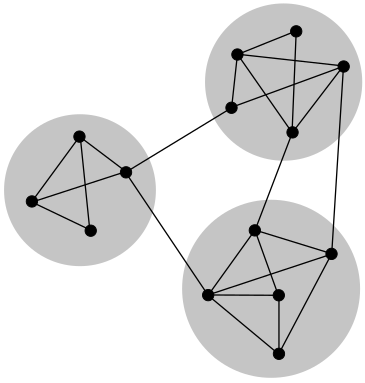
\includegraphics[scale=0.50]{img/community}
\caption{Esempio di una piccola rete nella quale {\`e} possibile visualizzare la struttura della comunit{\`a}, con tre gruppi di nodi con connessioni interne dense e connessioni pi{\`u} sparse tra i gruppi.}
\end{figure}

Un metodo di massimizzazione della modularit{\`a} {\`e} quello di Louvain \cite{louvain} che consiste di due fasi, ripetute in modo iterativo per massimizzare questo valore.

Innanzitutto, ciascun nodo nella rete {\`e} assegnato alla propria comunit{\`a}, favorendo le ottimizzazioni locali della modularit{\`a}. Per ogni nodo \( i \), viene calcolato il cambiamento di modularit{\`a} per rimuovere \( i \) dalla propria comunit{\`a} e spostarlo nella comunit{\`a} di ciascun suo vicino \( j \). Questo valore viene calcolato attraverso la seguente formula:

\begin{equation}
\Delta Q = \Biggl[ \frac{\sum_{in} + 2k_{i,in}}{2m} - \Biggl(\frac{\sum_{tot} + k_i}{2m} \Biggr)^2 \Biggr] - \Biggl[ \frac{\sum_{in}}{2m} - \Biggl(\frac{\sum_{tot}}{2m} \Biggr)^2 - \Biggl(\frac{k_i}{2m} \Biggr)^2 \Biggr]
\end{equation}

dove:

\begin{enumerate}[label=(\roman*)]
  
\item \( \sum_{in} \) {\`e} la somma di tutti i pesi degli archi all'interno della comunità nella quale \( i \) si sta muovendo;
\item \( \sum_{tot} \) {\`e}  la somma di tutti i pesi degli archi che coinvolgono i nodi della comunit{\`a};
\item \( k_i \) {\`e} il grado di \( i \);
\item {\`e} la somma dei pesi degli archi tra \( i \) e gli altri nodi nella comunit{\`a};
\item {\`e} la somma dei pesi di tutti gli archi del grafo.

\end{enumerate}

Una volta calcolato questo valore per tutte le comunit{\`a} a cui il nodo \( i \) {\`e} collegato, esso viene inserito nella comunit{\`a} che ha prodotto il maggiore aumento della modularit{\`a}. Se nessun aumento {\`e} possibile, il nodo \( i \) resta nella sua comunit{\`a} di partenza. Questo processo viene applicato ripetutamente e in sequenza a tutti i nodi fino a quando non si verifica un aumento della modularit{\`a}. Una volta raggiunto questo massimo locale di modularit{\`a}, la prima fase {\`a} terminata.

Nella seconda fase dell'algoritmo, tutti i nodi nella stessa comunit{\`a} vengono raggruppati e si crea una nuova rete in cui i nodi sono le comunit{\`a} della fase precedente. Tutti i collegamenti tra i nodi della stessa comunit{\`a} sono ora rappresentati da loop automatici sul nuovo nodo della comunità e i collegamenti da pi{\`u} nodi nella stessa comunità a un nodo in una comunit{\`a} diversa sono rappresentati da bordi ponderati tra le comunit{\`a}. Una volta creata la nuova rete, la seconda fase {\`e} terminata e la prima fase pu{\`o} essere riapplicata sulla nuova rete.

\section{Scoperta di Interazioni Basate su Frequenza}

Uno dei task tipici del data mining {\`e} quello di indagare la presenza di specifici aspetti frequenti in un archivio di dati. Questa necessit{\`a} ha le sue radici, come molti altri problemi, nella questione di dover profilare i comportamenti frequenti assunti da un agente a cui si {\`e} interessati. 

\subsection{Scoperta di Itemset Frequenti}
Il frequent itemset mining (o frequent patterns mining) {\`e} una delle aree di ricerca nell'ambito del data mining che si occupa nello specifico di offrire algoritmi e strutture dati che agevolino questo tipo di analisi.

Come il nome stesso suggerisce, il frequent patterns mining si occupa pertanto di indagare gli insiemi di oggetti che compaiono frequentemente insieme in una, pi{\`u} o meno grande, quantit{\`a} di dati: questo insieme di oggetti prende il nome di itemsets o di patterns frequenti.

\begin{defn}
Dato un insieme $I = \lbrace i_1, ..., i_n \rbrace$ di oggetti, si definisce k-itemset un qualsiasi sottinsieme $I_K \subseteq I$ di lunghezza $K (\lvert I_K \rvert = K)$.
\end{defn}

Generalmente c'{\`e} interesse soltanto per gli itemsets che esprimono caratteristiche particolari, nel caso del frequent itemset mining c'{\`e} interesse solo verso quelli che figurano un elevato numero di volte all'interno di un insieme di transazioni. 

\begin{defn}
Si definisce transazione i-esima \( T_i \) l'insieme $T_i \subseteq I$. Ciascuna transazione possiede un identificativo univoco \( i \).
\end{defn}

\begin{defn}
Dato un itemset \( I_k \), si dice che {\`e} contenuto in una transazione \( T_i \) se e sole se $I_k \subseteq T_i$.
\end{defn}

\begin{defn}
Si definisce database di transazioni l'insieme \( D \) delle transazioni \( T_i \).
\end{defn}

Intuitivamente {\`e} facile comprendere la notazione di frequenza, operativamente per{\`o} si necessita di una misura di confidenza in grado di suggerire quantitativamente se l'itemset considerato presenti effettivamente la caratteristica di ``essere frequente".

{\`E} possibile ricorrere a delle semplici statistiche per definire una che quantifichi la frequenza di un itemset in funzione di un livello di confidenza. 

In maniera abbastanza elementare {\`e} chiaro come, per un particolare itemset $I_k$ ci sia interesse nell'enumerare le transazioni $T_i$ che contengono $I_k$; nel gergo scientifico si usa dire che un itemset (o un patterns) ``copre" un determinato numero di transizioni.

\begin{defn}
Si definisce copertura di un itemset $I_k$ come l'insieme delle transazioni che lo includono:
\begin{equation}
coverage(I_k) = \lbrace T_i \in D \mid I_k \subseteq T_i \rbrace
\end{equation}
Chiaramente $coverage(I_k) \subseteq D$.
\end{defn}

Altrettanto sistematicamente, a partire dalla copertura, {\`e} possibile misurare il numero di transazioni che ``supportano" l'itemset.

\begin{defn}
Si definisce supporto assoluto di un itemset \( I_k \) come la cardinalit{\`a} della sua copertura:
\begin{equation}
support_{abs}(I_k) = \lvert coverage(I_k) \rvert
\end{equation}
Chiaramente il supporto {\`e} una misura discreta: $support_{abs}(I_k) \in \aleph$.
\end{defn}

Spesso al posto del supporto assoluto si usa il supporto relativo, una quantit{\`a} analoga che quantifica l'espressione della frequenza statistica di un itemset.

\begin{defn}
Si definisce supporto relativo di un itemset \( I_k \) come il rapporto del supporto assoluto ed il numero totale di transazioni nel database \( D \):
\begin{equation}
support_{rel}(I_k) = \frac{support_{abs}(I_k)}{ \lvert D \rvert } = \frac{ \lvert coverage(I_k) \rvert }{ \lvert D \rvert }
\end{equation}
Il supporto relativo {\`e} sempre compreso fra 0 e 1.
\end{defn}

Il supporto relativo {\`e}, a tutti gli effetti, il parametro che stabilisce la frequenza di un itemset ma, naturalmente, non stabilisce in maniera inequivocabile se sia frequente o infrequente.

La capacit{\`a} di attirbuire un valore di frequenza (o di infrequenza) ad un itemset {\`e} appannaggio esclusivo dell'operatore del task di data mining: uno stesso itemset \( I_k \) per un utente {\`e} da considerarsi frequente se copre il 20\% delle transazioni quando per un secondo utente potrebbe non essere cos{\`i}, ad esempio nel caso in cui debba coprire l'80\% delle transazioni. 

\begin{defn}
Un patterns \( I_k \) si dice frequente se $support_{rel}(I_K) > \alpha$ ove $\alpha$ {\`e} un valore di soglia minima stabilito dall'utente del task di mining.
\end{defn}

Avendo dato la definizione di supporto di un itemset occorre fare alcune particolari considerazioni: un database delle transazioni solitamente contiene pi{\`u} e pi{\`u} itemset differenti, che avranno un supporto altrettanto differente. Compito del frequent itemset mining {\`e} quello di scoprire tutti gli itemsets frequenti all'interno del database delle transazioni. 

Osservando il database delle transazioni pu{\`o} darci informazioni sull'insieme \( I \) degli oggetti ivi contenuti ma non sui k-itemsets di qualsiasi lunghezza.

Estrapolare questo tipo di informazione richiede un approccio di logica induttiva capace di trarre conclusioni su fatti specifici partendo da fatti pi{\`u} generali. 

Una strategia di ragionamento automatico del genere presuppone dei principi ben saldi di funzionamento che diano luogo ad uno spazio di ricerca facilmente esplorabile. Consideriamo l'esempio seguente: 

Dato un database \( D \) con 10 transazioni e dato l'insieme \( I = \lbrace a,b,c,d,e \rbrace \), per poter valutare tutti gli itemsets frequenti, in questo caso fino alla lunghezza massima di 5, dovremmo indagare in un insieme di $2^5$ combinazioni possibili.

\begin{figure}\centering
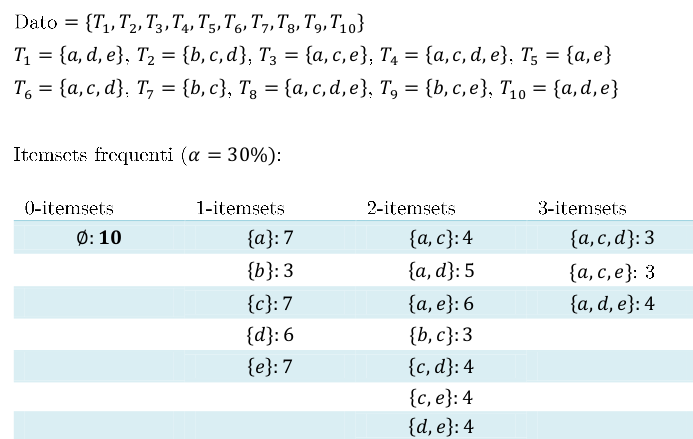
\includegraphics[scale=0.50]{img/itemsets}
\caption{Esempio di costruzione di k-itemsets a partire da un database di transazioni \( D \).}
\end{figure}

Lo stesso esempio suggerisce che, con la soglia del supporto indicata, il numero degli itemsets frequenti {\`e} pari a 16 con una lunghezza al pi{\`u} pari a 3: questo dovrebbe suggerire qualcosa.

Si {\`e} detto come il processo enumerativo di scoperta tenda a trarre conclusioni, per situazioni via via pi{\`u} specifiche a partire da situazioni pi{\`u} generali: questo {\`e} possibile mediante l'introduzione di una speciale relazione d'ordine sull'insieme degli itemsets.

\begin{defn}
Dati due itemsets \( I1 \) ed \( I2 \), si dice che \( I1 \) $\theta$-sussume \( I2 \) se e solo se esiste una sostituzione $\theta$ tale che \( I2 \) $\theta \subseteq I1$.
\end{defn}

\begin{defn}
Dati due itemsets \( I1 \) ed \( I2 \), allora \( I1 \) {\`e} pi{\`u} generale di \( I2 \) in sussunzione se e sole se \( I2 \) $\theta$-sussume $I1$; si scrive che $I1 \geq_{\theta} I2$.
\end{defn}

Tale definizione contribuisce a concretizzare lo spazio di ricerca, parzialmente ordinato per generalit{\`a}, dei $2^I$ patterns: il reticolo, o insieme parzialmente ordinato, $(2^I, \geq_{\theta})$.

\begin{figure}\centering
\label{img:8.2}
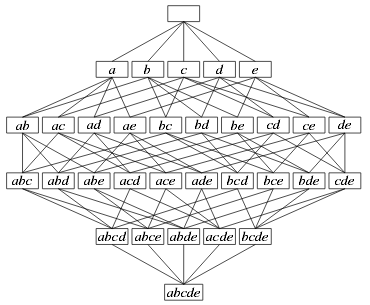
\includegraphics[scale=0.65]{img/reticolo-itemsets}
\caption{Diagramma di Hasse del reticolo $(2^I, \geq_{\theta})$ di tutti i possibili itemsets generabili nell'esercizio precedente.}
\end{figure}

Anche cos{\`i}, se si desiderasse trovare tutti e soli i frequenti bisognerebbe verificare esattamente tutti i possibili candidati: cercare nello spazio esponenziale di tutte le possibili combinazioni rende il problema velocemente intrattabile, {\`e} possibile ottimizzare la ricerca nel reticolo grazie ad una serie di propriet{\`a}:

\begin{enumerate}[label=(\roman*)]
  
\item propriet{\`a} di \textit{antimonotonicit{\`a}} del supporto: ad itemset pi{\`u} specifici, ossia quelli pi{\`u} in basso del reticolo, corrispondono supporti via via inferiori;

\begin{equation}
I_K \subset I_{K+h} \Rightarrow support_{rel}(I_K) > support_{rel}(I_{K+h})
\end{equation}

\item propriet{\`a} \textit{apriori}: nessuna specializzazione (superinsieme) di un itemset infrequente pu{\`o} essere frequente e, analogamente, tutti gli itemset pi{\`u} generali (sottoinsiemi) di un itemset frequente sono anch'essi frequenti.

\begin{equation}
support_{rel}(I_K) < \alpha \Rightarrow support_{rel}(I_{K+h}) < \alpha
\end{equation}

\end{enumerate}

Sfruttando tali propriet{\`a} {\`e} possibile costruire un approccio altamente enumerativo per la scoperta dei patterns frequenti. Tale tecninca consente di valutare solo gli itemsets direttamente frequenti, il tutto a partire dai pi{\`u} generali fino a terminare la ricerca con i pi{\`u} specifici: ricerca levelwise di tipo top-down.

\begin{figure}\centering
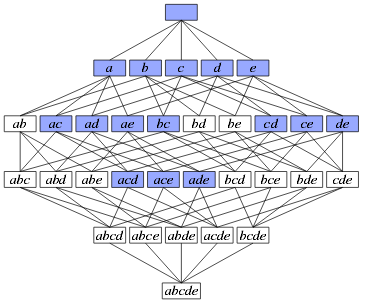
\includegraphics[scale=0.65]{img/reticolo-itemsets-frequenti}
\caption{Diagramma di Hasse del reticolo $(2^I, \geq_{\theta})$ di tutti i possibili itemsets generabili nell'esercizio precedente. Gli itemsets blu sono i soli frequenti: si noti come tengano le propriet{\`a} apriori e di antimonotonicit{\`a}.}
\end{figure}

In letteratura esistono diversi algoritmi di frequent itemset mining, fra i pi{\`u} celebri vi sono sicuramente apriori \cite{apriori} ed ECLAT \cite{eclat} che verranno citatati di seguito in quanto fondamentale per questo lavoro di tesi.

\subsection{Integrazione di Set Enumeration Tree}

In questa sezione si rivolgeranno delle brevi considerazioni ad una delle strutture dati utilizzate in letteratura per rappresentare il reticolo degli itemset $(2^I, \geq_{\theta})$. Guardando alla figura \ref{img:8.2} del paragrafo precedente si nota come, effettivamente, una struttura dati puramente reticolare risulterebbe difficile da mantenere in memoria e da gestire; l'insidia preponderante in questo tipo di questione {\`e} rappresentata dall'elevato numero di puntatori (archi) fra gli elementi ivi presenti. L'ideale sarebbe rocondurre una struttura reticolare ad una struttura dati basata sul concetto di albero.

Molti problemi informatici ammettono soluzioni i cui elementi appartengono ad un determinato insieme potenza. Nel caso del frequent itemset mining tale insieme potenza {\`e} proprio lo spazio \( 2^I \) dei possibili itemsets. L'idea chiave {\`e} quella di introdurre una struttura dati capace di operazioni di ricerca non ridondanti, ad esempio basata sulla riduzione degli archi. 

Nei problemi dove lo spazio di ricerca {\`e} un sottoinsieme dell'insieme potenza (nel caso del frequent itemset mining lo {\`e} l'insieme dei patterns frequenti ad esempio) chiuso per inclusione insiemistica {\`e} possibile utilizzare un set enumeration tree, meglio conosciuto come SE-Tree \cite{se-tree}.

Considerando come insieme base degli oggetti su cui enumerare gli itemset, l'insieme \( I \), si introduca al concetto di indice e di vista di un nodo.

\begin{defn}
Si definisce indice posizionale per gli oggetti $i \in I$ una funzione bigettiva del tipo $view:I \mapsto \aleph$.
\end{defn}

\begin{defn}
Dato l'insieme $S \subseteq I$ si definisce la vista di $S$ come l'insieme:
\begin{equation}
view(S) = \lbrace i \in I \mid index(i) > max_{j \in S}ind(j) \rbrace
\end{equation}
\end{defn}

La vista di un sottinsieme $S$ fornisce precise indicazioni di quali oggetti {\`e} possibile usare per poter espanderlo: nel reticolo, aumentando la lunghezza degli itemset, non si faceva altro che espandere un k-itemset, crearne cio{\`e} un superinsieme, sulla base di alcuni suoi 1-itemsets.

Si definisce un SE-Tree base, l'albero definito alla maniera seguente:

\begin{defn}
Sia \( F \) una collezione di insiemi su cui vale la chiusura per inclusione insiemistica, ossia $\forall$ \( S\) $\in$ \( F\) se \( S' \) $\subseteq$ \( S \) allora \( S' \) $\in$ \( F \), allora \( T \) {\`e} un SE-Tree per \( F \) se e solo se:

\begin{enumerate}[label=(\roman*)]
  
\item la radice di \( T \) {\`e} etichettata con l'insieme vuoto $\emptyset$;
\item i figli di un nodo etichettato con \( S \) in \( T \) sono dati dall'insieme \\ $\lbrace S \cup \lbrace e \rbrace \in F \mid e \in view(S) \rbrace$.

\end{enumerate}
\end{defn}

La definizione dice che un set enumeration tree per un insieme potenza (o insieme delle parti) {\`e} radicato nell'insieme vuoto e che i figli di ogni nodo sono risultati dall'unione di quel nodo con gli elementi di indice maggiore.

\begin{figure}\centering
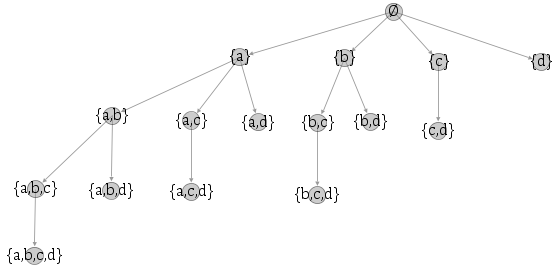
\includegraphics[scale=0.50]{img/se-tree}
\caption{SE-Tree dell'insieme $\lbrace a,b,c,d \rbrace$, questo SE-Tree potrebbe essere quello del reticolo degli itemsets costruibili a partire da $I = \lbrace a,b,c,d \rbrace$ secondo il reticolo $(2^I, \geq_{\theta})$.}
\end{figure}

Il set enumeration tree, possiede anche il carattere di albero dei prefissi: si noti come i nodi in relazione di discendenza condividano un prefisso via via crescente. Questo tipo di albero {\`e} chiaramente sbilanciato ma permette di valutare in maniera rapida la presenza di itemsets anche piuttosto grandi.

\subsection{Algoritmo ECLAT}

Nel frequent itemsets mining in generale molti algoritmi sfruttano a proprio vantaggio l'antimonotonicit{\`a} del supporto e la propriet{\`a} a priori; il tutto congiuntamente a strutture dati come il SE-Tree. 

Ai fini della tesi si studia molto brevemente un algoritmo di computazione degli itemset frequenti che getta le proprie basi su una versione insiemistica della regola a priori.

L'algoritmo ECLAT \cite{eclat} {\`e} un algoritmo efficiente di tipo top-down per la valutazione automatica degli itemset frequenti in un SE-Tree: significa che combina in qualche modo situazioni generali per trarre conclusioni su situazioni pi{\`u} specifiche.

ECLAT viene usato congiuntamente ad un SE-Tree per dedurre i patterns dal supporto elevato facendo un uso considerevole di intersezioni insiemistiche.

L'algoritmo funziona grazie ad un principio molto elementare, {\`e} certamente utile ed interessante considerare l'idea chiave alla base, anche chiamata ``propriet{\`a} ECLAT (Equivalent CLAss of Transactions)".

\begin{defn}
Dati due itemset \( I1 \) e \( I2 \) di uguale lunghezza \( k \), allora vale la seguente propriet{\`a}:

\begin{equation}
coverage( \langle I1,I2 \rangle ) = coverage(I1) \cap coverage(I2)
\end{equation}

\end{defn}

La propriet{\`a} di ECLAT {\`e} in accordo con la regola apriori, infatti si dimostra abbastanza banalmente che se \( I1 \) e \( I2 \) sono itemsets di lunghezza \( k \), allora \\ $I12 = \langle I1,I2 \rangle$ {\`e} un itemset di lunghezza \( k + 1 \), chiaramente risulta che:

\begin{equation}
\begin{split}
coverage(I12) = coverage(I1) \cap coverage(I2) \Rightarrow \\ 
\Rightarrow support_{abs}(I12) = \lvert coverage(I1) \cap coverage(I2) \rvert
\end{split}
\end{equation}
 
poich{\`e}:

\begin{equation}
\lvert coverage(I1) \cap coverage(I2) \rvert \leq min(support_{abs}(I1), support_{abs}(I2))
\end{equation}

allora vale:

\begin{equation}
support_{abs}(I12) \leq min \bigl( support_{abs}(I1),support_{abs}(I2) \bigr)
\end{equation}

In totale accordo con la regola di apriori: all'aumentare della lunghezza di un itemset il proprio supporto tende a decrescere.

Nel gergo dell'algoritmo l'insieme della copertura di un itemset prende il nome di tidlist (list of transaction ids) ma il funzionamento {\`e} veramente analogo. 

Sebbene rsultati sperimentali preferiscano ECLAT ad altri algoritmi di frequent itemset mining, le sue maggiori inefficienze sono quelle di richiedere numerose operazioni di intersezioni insiemistiche, inefficienti spesso sia in spazio che in tempo, oltre a richiedere di memorizzare una tidlist per ogni itemsets \footnote{Per grandi database di transazioni mantenere le tidlist (o le coperture) di ogni itemset pu{\`o} richiedere uno spreco enorme in memoria: l'uso di ECLAT {\`e} stato accuratamente valutato nel tempo anche in presenza di framework dinamici in grado di cambiare il tipo di rappresentazione delle tidlist per ragioni puramente di efficienza. Come se non bastasse l'aumento della dimensione delle tidlist favorisce una rapida degradazione delle performance al momento dell'intersezione.}.

\part{Esperimenti}
\chapter{Reddit}

\href{https://www.reddit.com/}{Reddit} {\`e} un aggregatore di social news nonch{\'e} sito internet di discussione e valutazione di contenuti web. Gli utenti registrati, chiamati redditors, possono pubblicare contenuti sotto forma di link o messaggi di testo che possono essere soggetti a commenti e a voti favorevoli o contrari da parte di altri membri, il che determina posizione e visibilit{\`a} dei vari contenuti sulle pagine del sito. Tali contenuti, chiamati discussions, vengono organizzati per argomenti in aree di interesse chiamate subreddits che coprono una variet{\`a} di argomenti tra cui istruzione, intrattenimento, humor, tecnologia, ecc..

\begin{figure}\centering

\includegraphics[scale=0.15]{img/reddit}
\caption{Logo di Reddit.}
\end{figure}

\subsection{Datasets}

I datasets mensili di Reddit, resi disonibili online in formato JSON dal author \href{https://www.reddit.com/users/Stuck_In_the_Matrix/}{u/Stuck\_In\_the\_Matrix} e suddivisi in \href{https://files.pushshift.io/reddit/discussions/}{discussions} (10 mln ca.) e \href{https://files.pushshift.io/reddit/comments/}{commenti} (80 mln ca.), sono stati importati all'interno di \href{https://www.mongodb.com/it}{MongoDB}, un DBMS\footnote{Database Management System} NoSQL orientato ai documenti, che ha permesso, per mezzo di indici di ricerca, una gestione pi{\`u} efficiente dei dati nei passi che verranno descritti in seguito.

\begin{figure}\centering

\includegraphics[scale=0.175]{img/mongo}
\caption{Logo di MongoDB.}
\end{figure}

\section{Filtraggio}

Per poter ridurre la dimensione dei dati in input ed allo stesso tempo dare un senso allo studio di cui parleremo in seguito, {\`e} stato effettuato un filtraggio per mezzo di alcuni criteri descritti nei paragrafi seguenti. A partire da quelle che sono le entit{\`a} del dominio applicativo in questione ci assicuriamo quindi di lavorare su un dataset formato da utenti particolarmente attivi e da discussions e commenti semanticamente significativi.

\subsection{Criteri}

\paragraph{Submissions}
Vengono considerati soltanto i discussions per cui:

\begin{enumerate}[label=(\roman*)]

\item
il numero di commenti {\`e} maggiore rispetto alla media, ossia:

\begin{equation}
\label{eq:1.1}
\text{\# commenti}>\frac{\text{\# commenti}}{\text{\# discussions}}
\end{equation}

\item
la lunghezza del selftext {\`e} maggiore rispetto alla media, ossia:

\begin{equation}
\label{eq:1.2}
\text{length(selftext)}>\frac{\sum_{s=1}^{\text{\# discussions}} \text{length(selftext(s))}}{\text{\# discussions}}
\end{equation}

\end{enumerate}

\paragraph{Commenti}
Vengono considerati soltanto i commenti per cui la lunghezza del body {\`e} maggiore rispetto alla media, ossia:

\begin{equation}
\text{length(body)}>\frac{\sum_{c=1}^{\text{\# commenti}} \text{length(body(c))}}{\text{\# commenti}}
\end{equation}

\paragraph{Redditors}
Vengono considerati soltanto i discussions ed i commenti scritti dai redditors in numero maggiore rispetto alla media, ossia:

\begin{equation}
\text{\# discussions + \# commenti}>\frac{\text{\# discussions + \# commenti}}{\text{\# distinti utenti}}
\end{equation}

\paragraph{Subreddits}
Vengono considerati soltanto i subreddits per cui il numero di discussions appartenenti, in seguito al filtraggio definito dai criteri \eqref{eq:1.1} e \eqref{eq:1.2}, risulti maggiore rispetto alla media, ossia:

\begin{equation}
\text{\# discussions filtrati}>\frac{\text{\# discussions}}{\text{\# distinti subreddit}}
\end{equation}

In riferimento al dataset Reddit di Novembre 2017, ad esempio, i criteri appena definiti hanno prodotto un filtraggio dei dati come segue. Vengono considerati:

\begin{enumerate}[label=(\roman*)]

\item 
i \textit{discussions} per cui il numero di commenti {\`e} maggiore di 8 e per cui la lunghezza del selftext {\`e} maggiore di 168 caratteri;

\item
i \textit{commenti} per cui la lunghezza del body {\`e} maggiore di 170 caratteri;

\item 
i discussions ed i commenti che i \textit{redditors} autori hanno scritto in numero maggiore di 20;

\item
i \textit{subreddits} per cui il numero di discussions che vi appartengono, in seguito al filtraggio, {\`e} maggiore di 77.

\end{enumerate}

I dati sono stati modellati optando per una rappresentazione ad albero dei subreddits che rispecchiasse la struttura del dominio applicativo dovuta alla possibilit{\`a} di interazioni multi-threading tra i redditors sotto un determinato submission. In dettaglio: un documento della nuova collezione rappresenta un subreddit con relativo id e nome. Ogni subreddit contiene una lista di discussions che, a loro volta, possono contenere una lista di commenti. Ogni submission e/o commento contiene un id, l'autore, la data e l'ora della pubblicazione ed il risultato della fase di NLP sul corpo testuale. Ogni submission contiene una lista di similarit{\`a} lessicali e semantiche calcolate come definito nelle sezioni precedenti ed ogni commento pu{\`o} a sua volta contenere un'altra lista di commenti con gli stessi campi e cos{\`i} via per oguno di essi.

\newpage

\lstinputlisting[language=json, caption={Esempio di JSON Subreddit}, captionpos=b]{sample.json}

A partire da oggetti Java creati per mezzo di classi modellate opportunamente per poter rappresentare le entit{\`a} del social media Reddit cos{\`i} come sopra descritte, {\`e} stato possibile, grazie alle \href{https://github.com/google/gson}{API Gson} di Google, convertire tali oggetti in documenti JSON che sono poi stati serializzati all'interno di una nuova collezione di MongoDB. 
% \chapter{Risultati Sperimentali}

\section{Risultati Quantitativi}

\section{Risultati Qualitativi}

\begin{thebibliography}{9}

\bibitem{hic} Fu, Tianjun, Ahmed Abbasi, and Hsinchun Chen. ``A hybrid approach to web forum interactional coherence analysis." Journal of the Association for Information Science and Technology 59.8 (2008): 1195-1209.

\bibitem{lin} Lin, Dekang. ``An information-theoretic definition of similarity." Icml. Vol. 98. No. 1998. 1998.

\bibitem{Bavelas-centrality} Bavelas, Alex. ``A mathematical model for group structures." Human organization 7.3 (1948): 16-30.

\bibitem{Sabidussi-centrality} Sabidussi, Gert. ``The centrality index of a graph." Psychometrika 31.4 (1966): 581-603.

\bibitem{Freeman-centrality} Freeman, Linton C. ``Centrality in social networks conceptual clarification." Social networks 1.3 (1978): 215-239.

\bibitem{Anthonisse-betweenness} Anthonisse, Jac M. ``The rush in a directed graph." Stichting Mathematisch Centrum. Mathematische Besliskunde BN 9/71 (1971).

\bibitem{Freeman-betweenness} Freeman, Linton C. ``A set of measures of centrality based on betweenness." Sociometry (1977): 35-41.

\bibitem{Brandes-betweenness} Brandes, Ulrik. ``A faster algorithm for betweenness centrality." Journal of mathematical sociology 25.2 (2001): 163-177. 

\bibitem{louvain} Blondel, Vincent D., et al. ``Fast unfolding of communities in large networks." Journal of statistical mechanics: theory and experiment 2008.10 (2008): P10008.

\bibitem{apriori} Agarwal, Rakesh, and Ramakrishnan Srikant. ``Fast algorithms for mining association rules." Proc. of the 20th VLDB Conference. 1994.

\bibitem{eclat} Zaki, Mohammed Javeed, et al. ``New Algorithms for Fast Discovery of Association Rules." KDD. Vol. 97. 1997.

\bibitem{se-tree} Rymon, Ron. ``Search through systematic set enumeration." (1992).

\end{thebibliography}


\end{document}
